\chapter{Solving Recurrences}

\section{The Master Theorem}

If $T(n) = aT(\frac{n}{b}) + O(n^d)$, then

\begin{math}
T(n) = \left\{
\begin{array}{l l}
O(n^d)       & \quad \text{if} d > log_ba \\
O(n^d logn)  & \quad \text{if} d = log_ba \\
O(n^{log_ba}) & \quad \text{if} d < log_ba \\
\end{array} \right.
\end{math}

\section{Recursion Tree}

We can reason about a recurrence of the form: $ T(n) = aT(\frac{n}{b})
+ f(n) $ where $ a \geq 0, b > 0 $ with the following recursion tree:

{
  % Current graphic is hand-drawn by John Howat.
  % Should replace asap with a nicer diagram
  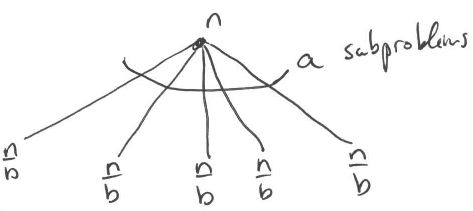
\includegraphics[scale=1.2]{recursion_tree}
  %\caption{A recursion tree representing a recursions on n/b elements}
  \label{fig:recursion_tree}
}
